%!TEX root = main.tex
\subsection{Dynamic Panel Example}
\label{sec:Dpanel_sim}
We now consider two simulation experiments based on section \ref{sec:Dpanel}, applying the GFIC to a dynamic panel model. 
For both experiments our data generating process is similar to that of \cite{AndrewsLu}, specifically
	\begin{equation}
	\label{eq:covar}
		\left[\begin{array}{c}
			x_{i}\\
			\eta_i\\
			v_{i}
  \end{array} \right]\sim \mbox{iid}\; N\left(\left[\begin{array}{c}\mathbf{0}_T\\ 0\\ \mathbf{0}_T \end{array}\right] ,\left[\begin{array}{ccc}
	 	 I_T & \sigma_{x\eta}\iota_T&\sigma_{xv}\Gamma_T \\
     \sigma_{x\eta}\iota_T'& 1&\mathbf{0}_T' \\
     \sigma_{xv}\Gamma_T'& \mathbf{0}_T&  I_T
	 \end{array}\right]\right)
	\end{equation}
where $\mathbf{0}_m$ denotes an $m$-vector of zeros, $I_m$ the $(m\times m)$ identity matrix, $\iota_m$ an $m$-vector of ones, and $\Gamma_m$ an $m\times m$ matrix with ones on the subdiagonal and zeros elsewhere, namely
	\begin{equation}
		\Gamma_m = \left[\begin{array}{cc}
        \mathbf{0}_{m-1}' & 0\\
        I_{m-1} & \mathbf{0}_{m-1}
	 \end{array}\right].
	\end{equation}
Under this covariance matrix structure $\eta_i$ and $v_{i}$ are uncorrelated with each other, but both are correlated with $x_{i}$: $E[x_{it}\eta_i]=\sigma_{x\eta}$ and $x_{it}$ is predetermined but not strictly exogenous with respect to $v_{it}$. Specifically, $E[x_{it}v_{it-1}]=\sigma_{xv}$, while $E[x_{it}v_{is}]=0$ for $s\neq t-1$. 
We initialize the pre-sample observations of $y$ to zero, the mean of their stationary distribution, and generate the remaining time periods according to Equation \ref{eq:truepanel} with $\theta = 0.5$ and $\sigma_{x\eta} = 0.2$.
The true lag length differs in our two examples as does the target parameter, so we explain these features of the simulation designs below. 
Unlike \cite{AndrewsLu} we do not generate extra observations to keep the time dimension fixed across estimators with different lag specifications.
This is for two reasons. 
First, in real-world applications such additional observations would not be available. 
Second, we are explicitly interested in trading off the efficiency gain from including additional time periods in estimation against the bias that arises from estimating an incorrect lag specification. 

\subsubsection{Long-run versus Short-run Effects}
\label{sec:SRvsLR}
Consider two different researchers who happen to be working with the same panel dataset. 
One wishes to estimate the short-run effect of $x$ on $y$ while the other wishes to estimate the long-run effect.  
Should they use the same model specification?
We now present an example showing that the answer, in general, is no.
Suppose that the true model is
\[
  y_{it} = \theta x_{it} + \gamma_1 y_{it-1} + \gamma_2 y_{it-2}  + \eta_i + v_{it}
\]
where $i = 1, \dots, n = 250$ and $t = 1, \dots, T=5$ and the regressor, individual effect and error term are generated according to Equation \ref{eq:covar}, as described in the preceding section.
Our model selection decision in this example is whether to set $\gamma_2 = 0$ and estimate a specification with one lag only.
We denote this one-lag specification by $\mbox{L1}$ and the true specification, including both lags, by $\mbox{L2}$.
To focus on the model selection decision, we fix the instrument set in this experiment to $\mathbf{z}_{it}(\ell,\text{P})$, defined in Equation \ref{eq:Zdpanel}.
Because this instrument set is valid when $x$ is pre-determined, it does not introduce bias into our estimation.
Thus, bias only emerges if we estimate $\mbox{L1}$ when $\gamma_2\neq 0$.
Our simulation design takes $\theta = 0.5, \gamma_1 = 0.4, \sigma_{x\eta} = 0.2$, and $\sigma_{xv} = 0.1$ and varies $\gamma_2$ over the range $\{0.10, 0.11, \dots, 0.19, 0.20\}$. 

Table \ref{tab:MAD_SRvsLR} presents the results of the simulation, based on 1000 replications at each grid point.
Because they are based on \emph{ratios} of estimators of $\theta$ and $\gamma_1, \gamma_2$, estimators of the long-run effect may not have finite moments, making finite-sample MSE undefined.
The usual solution to this problem in simulation settings is to work with so-called ``trimmed'' MSE by discarding observations that fall outside, say, a range $[-M, M]$ before calculating MSE.\footnote{Note that \emph{asymptotic} MSE remains well-defined even for estimators that do not possess finite-sample moments so that GFIC comparisons remain meaningful. By taking the trimming constant $M$ to infinity, one can formalize the notion that asymptotic MSE comparisons can be used to ``stand in'' for finite-sample MSE even when the latter does not exist. For more details, See \cite{HansenShrink} and online appendix C of \cite{DiTraglia2016}.}
Because there is no clear way to set the trimming constant $M$, it can be difficult to interpret results based on trimmed MSE unless they consider multiple values of $M$.
To avoid this issue, Table \ref{tab:MAD_SRvsLR} reports simulation results for median absolute deviation (MAD).
Results for trimmed MSE with different choices of $M$ are similar and are available upon request.

\begin{table}[!hpt]
\centering
\small
\begin{tabular}{  c  c c  c  c c c  }
\hline
\hline
 & \multicolumn{3}{c}{Short-run Effect} & \multicolumn{3}{c}{Long-run Effect} \\
    $\gamma_2$ &      L2  &       L1   &    GFIC    & L2 &     L1 &   GFIC\\
    \hline
 0.10  &0.231&\bf{\color{blue}0.141}& 0.173& 0.801& \bf{\color{blue}0.582}& 0.688\\
  0.11 & 0.237& \bf{\color{blue}0.156}& 0.181& 0.834& \bf{\color{blue}0.633}& 0.716\\
 0.12   &0.240& \bf{\color{blue}0.174}& 0.193& 0.850& \bf{\color{blue}0.685}& 0.752\\
 0.13   &0.238& \bf{\color{blue}0.187}& 0.201& 0.870& \bf{\color{blue}0.729}& 0.787\\
 0.14 &0.220& \bf{\color{blue}0.198}& 0.203& 0.870& \bf{\color{blue}0.764}& 0.808\\
\bf{\color{red} 0.15}  & \bf{\color{blue}0.201}& 0.219& 0.211& 0.844& \bf{\color{blue}0.822}& 0.839\\
\bf{\color{red} 0.16}  & \bf{\color{blue}0.205}& 0.223& 0.210& 0.883& \bf{\color{blue}0.856}& 0.862\\
 0.17  &\bf{\color{blue}0.181}& 0.242& 0.204& \bf{\color{blue}0.860}& 0.911& 0.897\\
 0.18  & \bf{\color{blue}0.162}& 0.258& 0.189& \bf{\color{blue}0.835}& 0.959& 0.891\\
 0.19  &\bf{\color{blue}0.161}& 0.265& 0.181& \bf{\color{blue}0.866}& 0.997& 0.917\\
 0.20  &\bf{\color{blue}0.143}& 0.288& 0.162& \bf{\color{blue}0.858}& 1.054& 0.910 \\
\hline
 \hline
\end{tabular}
\caption{Comparisons of mean absolute deviation (MAD) for estimators of the Short-run and Long-run effects of $x$ on $y$ in the simulation experiment described in Section \ref{sec:SRvsLR}.
The columns labeled $\mbox{L1}$ and $\mbox{L2}$ give the MAD of estimators that fix the lag length to one and two, while the columns labeled GFIC give the MAD of an estimator that selects lag length via the GIFC.
Results are based on 1000 simulation replications from the DGP described in Section \ref{sec:Dpanel_sim} with $\gamma_1 = 0.4$, using the estimators described in Section \ref{sec:Dpanel} and the instrument set $\mathbf{z}_{it}(\ell, \text{P})$ from Equation \ref{eq:Zdpanel}.}
\label{tab:MAD_SRvsLR}
\end{table}		

The columns of Table \ref{tab:MAD_SRvsLR} labeled $\mbox{L1}$ and $\mbox{L2}$ give the MAD of estimators that fix the lag length to one and two, while those labeled GFIC give the MAD of an estimator that selects lag length via the GFIC.
Notice that throughout the table $\gamma_2 \neq 0$ so that $\mbox{L1}$ is \emph{mis-specified}.
Nonetheless, $\mbox{L1}$ yields lower MAD estimators of both the short-run and long-run effects when $\gamma_2$ is sufficiently small and the difference can be substantial.
When $\gamma_2 = 0.2$, for example, MAD for is 0.582 for the long-run effect estimator based on $\mbox{L1}$ versus 0.801 for that based on $\mbox{L2}$.
Note moreover that point at which $\gamma_2$ becomes large enough for $\mbox{L2}$ to be preferred depends on which effect we seek to estimate.
When $\gamma_2$ equals 0.15 or 0.16, $\mbox{L1}$ gives a lower MAD for the short-run effect while $\mbox{L2}$ gives a lower MAD for the long-run effect.
Because it chooses between $\mbox{L1}$ and $\mbox{L2}$ and is subject to random model selection errors, the GFIC can never outperform the oracle estimator that uses $\mbox{L1}$ when it is optimal in terms of MAD and $\mbox{L2}$ otherwise.
Instead, the GFIC represents a compromise between two extremes: its MAD is never as large as that of the worst specification and never as small as that of the best specification.
When there are large MAD differences between $\mbox{L1}$ and $\mbox{L2}$, however, GFIC is generally quite close to the optimum.


\subsubsection{Simultaneous Model and Moment Selection for the Short-run Effect}
\todo[inline]{This needs to be cleaned up. Introduce it by saying something like: now a more substantial simulation that focuses on the short-run effect as in our empirical example below. Also need to add the new tables and figures that I made.}

In the simulation we take $\theta = 0.5$, $\sigma_{x\eta}=0.2$ and vary $\gamma$, $\sigma_{xv}$, $T$ and $N$ over a grid.
Each grid point is based on 2000 simulation replications.

The first question is how the finite sample MSE of the 2SLS estimators of $\theta$ based on specifications LW, LS, W, and S (see Section \ref{sec:Dpanel}) changes with $\gamma$ and $\sigma_{xv}$. 
Figures \ref{fig:best} and \ref{fig:advantage} present RMSE comparisons for these four estimators over a simulation grid with $\gamma, \sigma_{xv} \in \{0, 0.005, 0.01, \hdots, 0.195, 0.2\}$, $N \in \{250,500\}$, $T \in \{4,5\}$.\footnote{Taking $T$ no smaller than 4 ensures that MSE exists for all four estimators: the finite sample moments of the 2SLS estimator only exist up to the order of over-identification.} 
For each point in the parameter space, the color in Figure \ref{fig:best} indicates the estimator of $\theta$ with the \emph{lowest} finite sample RMSE. 
The saturation of the color indicates the relative difference in RMSE of the best estimator at that point measured against the second-best estimator: darker indicates a larger advantage; lighter indicates a smaller advantage. 
While Figure  \ref{fig:best} indicates \emph{which} estimator is best, Figure \ref{fig:advantage} indicates how much of an advantage in RMSE can be gained over the correct specification, LW. 
These plots indicate that, provided $\gamma$ and $\sigma_{xv}$ are not too large, there are potentially large gains to be had by intentionally using an incorrectly specified estimator. 
The question remains, can the GFIC identify such situations?

%%%%%%%%%%%%%%%%%%%%%%%%%%%%%%%%%%%%%%%%
\begin{figure}
\centering
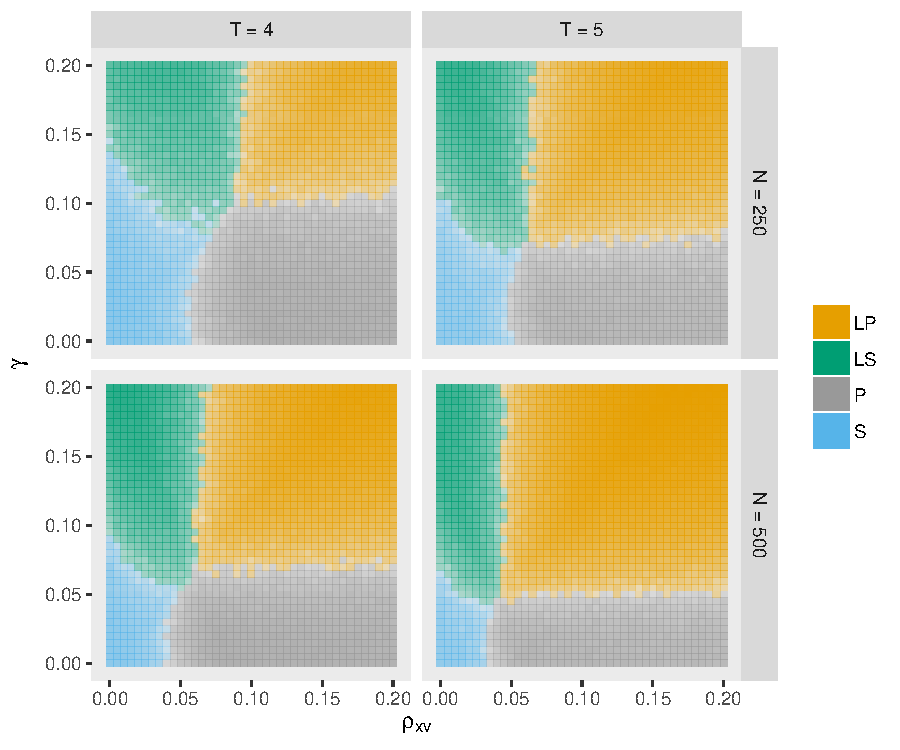
\includegraphics[scale = 0.8]{./simulations/DynamicPanel/results/Dpanel_oracle}
\caption{ Minimum RMSE Specification at each combination of parameter values. Shading gives RMSE relative to second best specification.}
\label{fig:best}
\end{figure}
%%%%%%%%%%%%%%%%%%%%%%%%%%%%%%%%%%%%%%%%
\begin{figure}
\centering
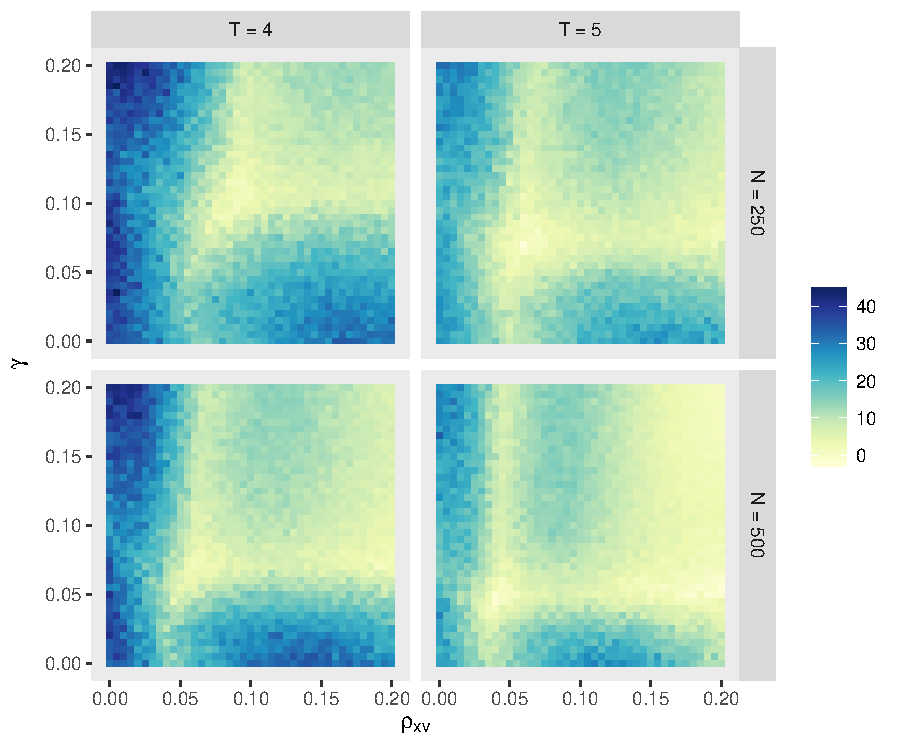
\includegraphics[scale = 0.8]{./simulations/DynamicPanel/results/Dpanel_GFIC_RMSE_rel_oracle}
\caption{GFIC RMSE relative to Oracle}
\end{figure}
%%%%%%%%%%%%%%%%%%%%%%%%%%%%%%%%%%%%%%%%
\begin{figure}
\centering
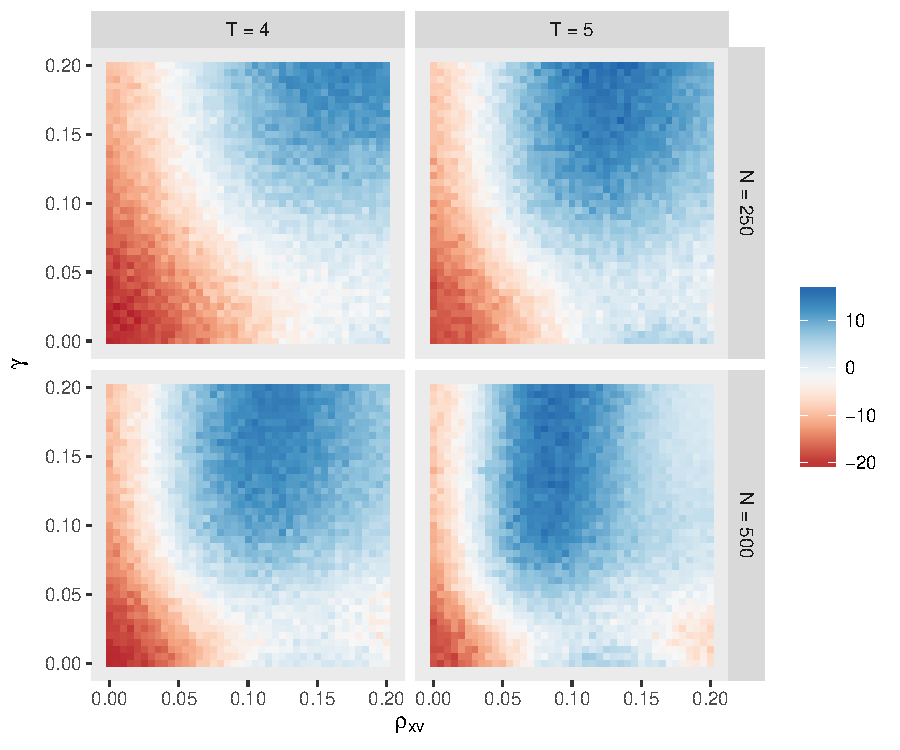
\includegraphics[scale = 0.8]{./simulations/DynamicPanel/results/Dpanel_GFIC_RMSE_rel_LP}
\caption{GFIC RMSE relative to LP}
\end{figure}
%%%%%%%%%%%%%%%%%%%%%%%%%%%%%%%%%%%%%%%%
\begin{figure}
\centering
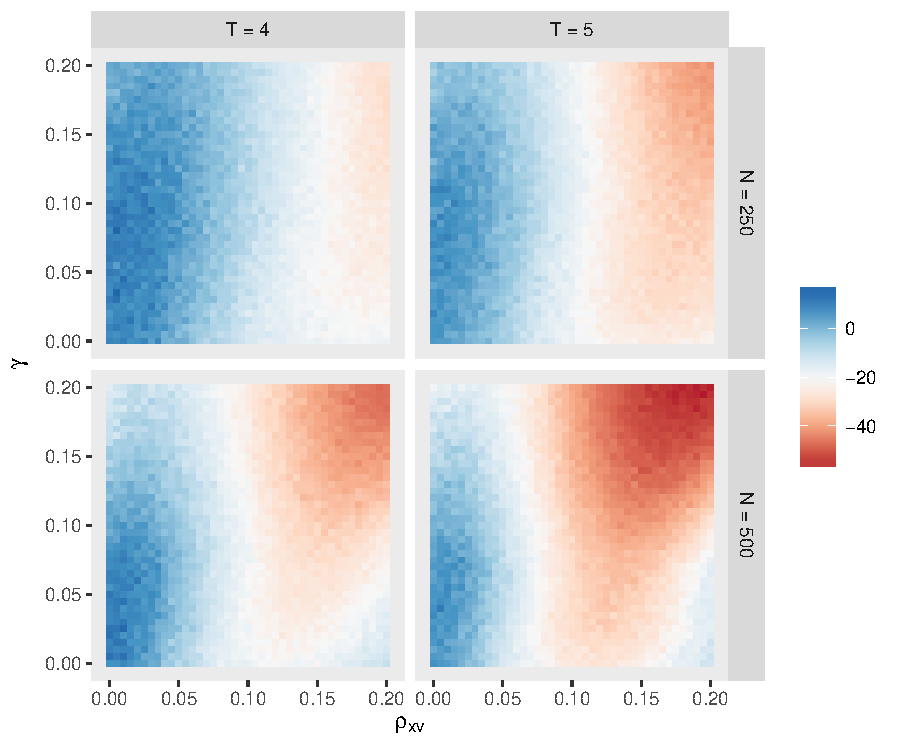
\includegraphics[scale = 0.8]{./simulations/DynamicPanel/results/Dpanel_GFIC_RMSE_rel_AIC}
\caption{GFIC RMSE relative to AIC}
\end{figure}
%%%%%%%%%%%%%%%%%%%%%%%%%%%%%%%%%%%%%%%%
\begin{figure}
\centering
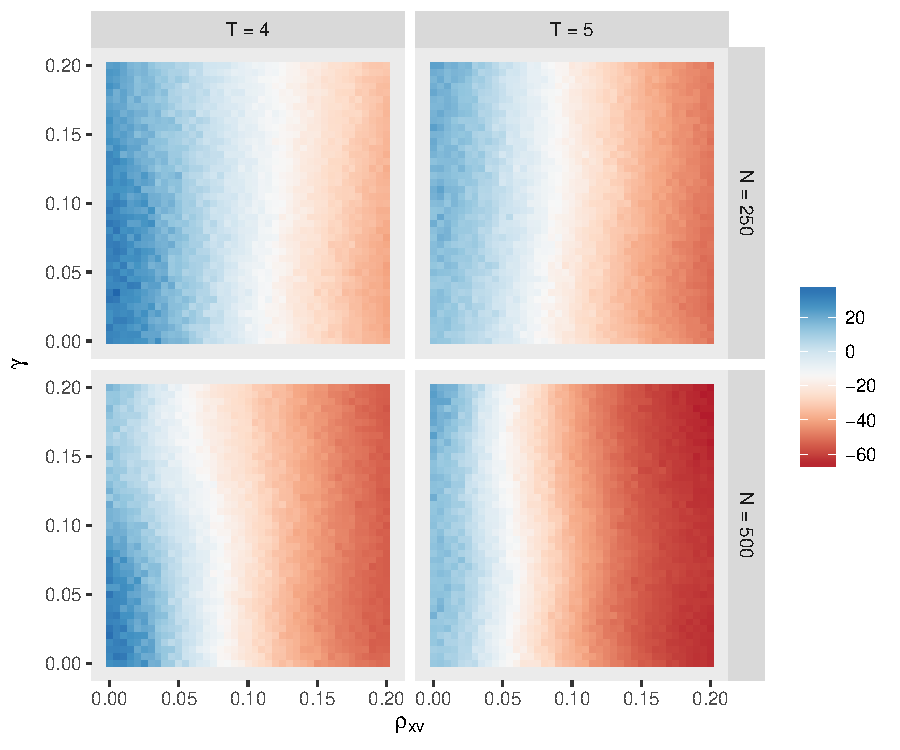
\includegraphics[scale = 0.8]{./simulations/DynamicPanel/results/Dpanel_GFIC_RMSE_rel_BIC}
\caption{GFIC RMSE relative to BIC}
\end{figure}
%%%%%%%%%%%%%%%%%%%%%%%%%%%%%%%%%%%%%%%%
\begin{figure}
\centering
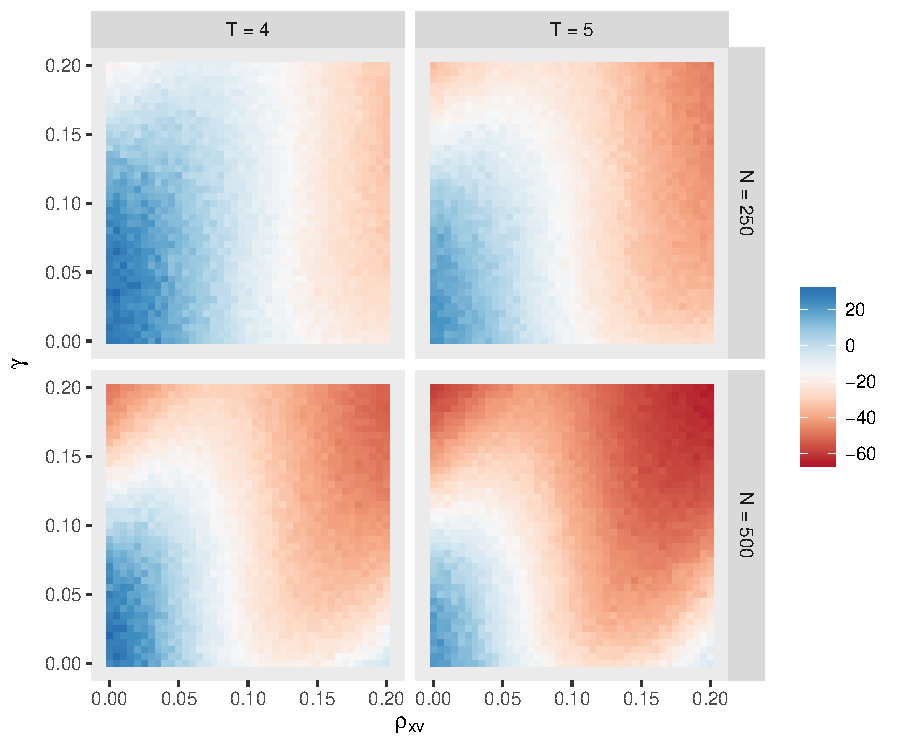
\includegraphics[scale = 0.8]{./simulations/DynamicPanel/results/Dpanel_GFIC_RMSE_rel_J5}
\caption{GFIC RMSE relative to J5}
\end{figure}
%%%%%%%%%%%%%%%%%%%%%%%%%%%%%%%%%%%%%%%%
\begin{figure}
\centering
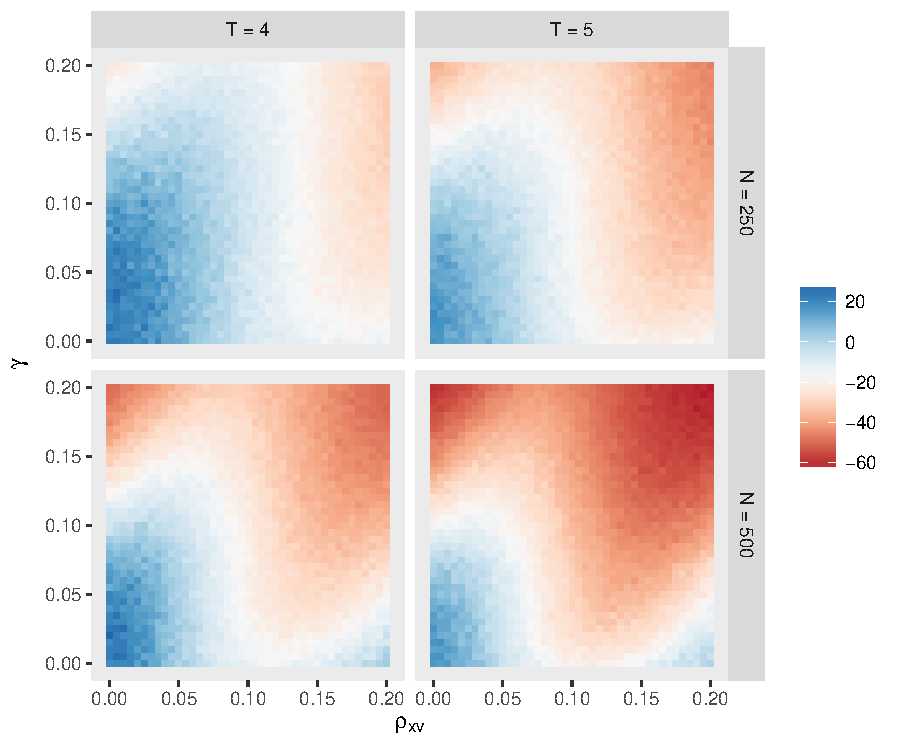
\includegraphics[scale = 0.8]{./simulations/DynamicPanel/results/Dpanel_GFIC_RMSE_rel_J10}
\caption{GFIC RMSE relative to J10}
\end{figure}

%%%%%%%%%%%%%%%%%%%%%%%%%%%%%%%%%%%%%%%%
\begin{figure}
\centering
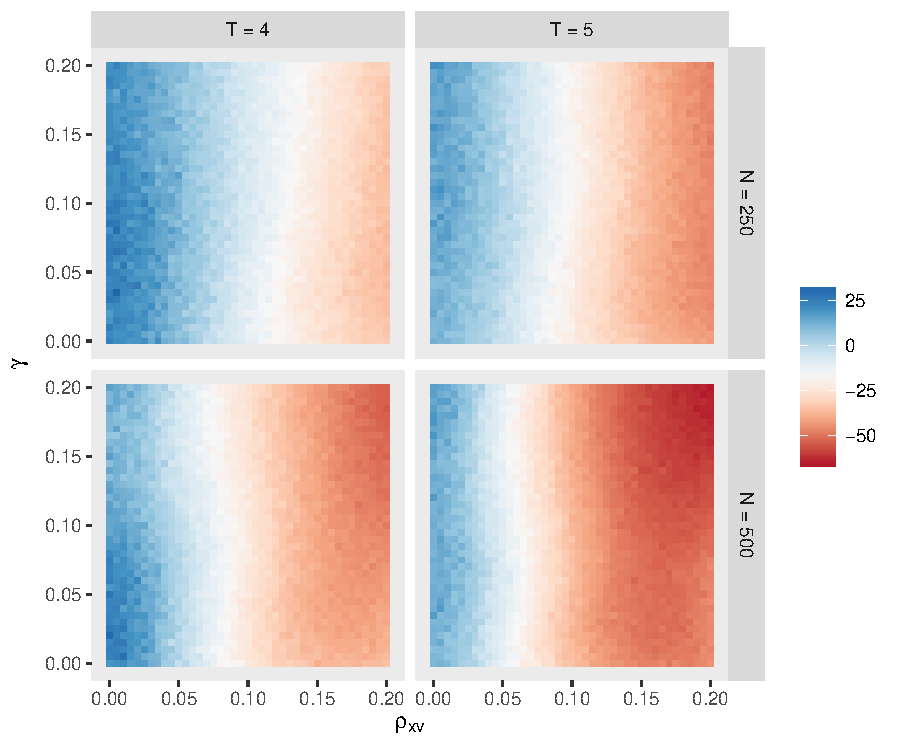
\includegraphics[scale = 0.8]{./simulations/DynamicPanel/results/Dpanel_GFIC_RMSE_rel_HQ}
\caption{GFIC RMSE relative to HQ}
\end{figure}

%%%%%%%%%%%%%%%%%%%%%%%%%%%%%%%%%%%%%%%%
\begin{figure}
\centering
\caption{Here's where the old figure used to be!}
\label{fig:advantage}
\end{figure}

%%%%%%%%%%%%%%%%%%%%%%%%%%%%%%%%%%%%%%%%

To provide a basis for comparison, we consider a number of other selection procedures. 
The first is a ``na\"{i}ve'' Downard J-test. 
To implement this procedure, we select the \emph{most restrictive} specification that is not rejected by the over-identifying restrictions test at a fixed significance level, either 5\% or 10\%. 
Specifically, we proceed as follows:
\begin{enumerate}
\item Use S unless the J-test rejects it. 
\item If S  is rejected, use W unless the J-test rejects it. 
\item If W is rejected, use LS unless the J-test rejects it. 
\item Only use LW if all others specifications are rejected.
\end{enumerate}
This procedure is ``na\"{i}ve'' because the significance thresholds are chosed arbitrarily rather than with a view towards some kind of selection optimality. 
We also consider the GMM model and moment selection criteria of \cite{AndrewsLu}: 
	\begin{eqnarray*}
	 \mbox{GMM-BIC} && J - (|c| - |b|) \log{n}\\
	 \mbox{GMM-AIC}&& J - 2(|c| - |b|)\\ 
	 \mbox{GMM-HQ} && J - 2.01 (|c| - |b|)  \log{\log{n}}
	\end{eqnarray*}
where $|b|$ is the number of parameters estimated, and $|c|$ the number of moment conditions used. 
Under certain assumptions, it can be shown that both the GMM-BIC and GMM-HQ are consistent: they select the maximal correctly specified estimator with probability approaching one in the limit. 
To implement these criteria, we calculate the J-test based on the optimal, two-step GMM estimator with a panel robust, heteroscedasticity-consistent, centered covariance matrix estimator for each specification.

To compare selection procedures we use the same simulation grid as above, namely $\gamma$ and $\sigma_{xv}$, namely $\gamma, \sigma_{xv} \in \{0, 0.005, 0.01, \hdots, 0.195, 0.20\}$.  
Again, each point on the simulation grid is calculated from 2000 simulation replications. 
Tables \ref{tab:rel} and \ref{tab:rmse} compare the performance of GFIC selection against each of the fixed specifications LW, LS, W, and S as well as the Downward J-test and the GMM moment and model selection criteria of \cite{AndrewsLu}. 
Table \ref{tab:rmse} gives average and maximum, i.e.\ worst-case, RMSE over the parameter space for $\gamma, \sigma_{xv}$ while Table \ref{tab:rel} gives \emph{relative} RMSE comparisons. Specifically, the values in the panel ``Average'' of Table \ref{tab:rel} tell how much larger, in percentage points, the average RMSE of a given estimator or selection procedure is than that of the pointwise oracle. 
The pointwise oracle is the infeasible procedure that uses the true minimum RMSE estimator at each point on the parameter grid. 
In contrast, the values in the panel ``Worst-Case'' of Table \ref{tab:rel} tell how much larger, in percentage points, the maximum RMSE of a given estimator or selection procedure is than that of the fixed specification LW. 
Over this parameter grid, LW is the minimax estimator.

Compared both to the fixed specifications and the other selection procedures, the GFIC performs well. 
In particular, it has a substantially lower average and worst-case RMSE than any of the other selection procedures.
Compared to simply using the correct specification, LW, the GFIC also performs relatively well. 
When $T$ and $N$ are small, the GFIC outperforms LW in average RMSE. 
As they grow it performs slightly worse, but only by a small amount.


\begin{table}[!tbp]
  \centering
\caption{This is where the old table used to be!}
\label{tab:rel}
\end{table}

%%%%%%%%%%%%%%%%%%%%%%%%%%%%%%%%%%%%%%%%

\begin{table}[!tbp]
  \centering
\caption{This is where the old table used to be!}
\label{tab:rmse}
\end{table}
%%%%%%%%%%%%%%%%%%%%%%%%%%%%%%%%%%%%%%%%
\begin{sidewaystable}
  \footnotesize
  \centering
  \begin{tabular}{cccc|cccc|cccc|cccc|cccc|cccc} 
 \hline \hline 
\multicolumn{4}{c}{}&\multicolumn{4}{c}{GFIC}&\multicolumn{4}{c}{LP}&\multicolumn{4}{c}{LS}&\multicolumn{4}{c}{P}&\multicolumn{4}{c}{S}\\ 
 \hline
 &  &  & $\rho$ & 0 & 0.05 & 0.1 & 0.15 & 0 & 0.05 & 0.1 & 0.15 & 0 & 0.05 & 0.1 & 0.15 & 0 & 0.05 & 0.1 & 0.15 & 0 & 0.05 & 0.1 & 0.15 \\
$T$ & $N$ & $\gamma$ &  &  &  &  &  &  &  &  &  &  &  &  &  &  &  &  &  &  &  &  &  \\
\hline
4 & 250 & 0 &  & 57 & 60 & 62 & 67 & 72 & 70 & 69 & 68 & 51 & 58 & 74 & 95 & 51 & 53 & 52 & 52 & 42 & 49 & 65 & 86 \\
 &  & 0.05 &  & 60 & 62 & 67 & 69 & 74 & 71 & 71 & 70 & 52 & 59 & 77 & 95 & 58 & 57 & 58 & 56 & 43 & 54 & 72 & 91 \\
 &  & 0.1 &  & 66 & 67 & 74 & 75 & 77 & 72 & 74 & 71 & 52 & 57 & 76 & 97 & 76 & 73 & 71 & 70 & 47 & 60 & 77 & 97 \\
 &  & 0.15 &  & 71 & 75 & 78 & 82 & 81 & 77 & 74 & 75 & 53 & 62 & 76 & 99 & 99 & 96 & 92 & 89 & 55 & 69 & 84 & 103 \\
 \hline
 & 500 & 0 &  & 40 & 43 & 48 & 48 & 51 & 49 & 49 & 48 & 37 & 47 & 67 & 90 & 37 & 37 & 36 & 36 & 30 & 40 & 59 & 83 \\
 &  & 0.05 &  & 43 & 47 & 51 & 49 & 52 & 50 & 51 & 49 & 36 & 47 & 67 & 90 & 45 & 45 & 44 & 43 & 31 & 47 & 65 & 87 \\
 &  & 0.1 &  & 45 & 53 & 56 & 54 & 52 & 51 & 50 & 50 & 36 & 47 & 69 & 90 & 67 & 64 & 62 & 59 & 37 & 53 & 73 & 92 \\
 &  & 0.15 &  & 50 & 56 & 59 & 56 & 56 & 53 & 52 & 50 & 36 & 48 & 69 & 92 & 92 & 90 & 85 & 83 & 45 & 63 & 80 & 100 \\
 \hline
5 & 250 & 0 &  & 45 & 48 & 54 & 56 & 56 & 56 & 55 & 54 & 42 & 51 & 70 & 91 & 44 & 45 & 44 & 45 & 36 & 44 & 62 & 83 \\
 &  & 0.05 &  & 48 & 52 & 56 & 55 & 58 & 56 & 55 & 54 & 43 & 52 & 70 & 92 & 52 & 51 & 51 & 48 & 38 & 50 & 68 & 89 \\
 &  & 0.1 &  & 51 & 57 & 61 & 58 & 59 & 57 & 55 & 55 & 44 & 53 & 72 & 94 & 68 & 66 & 65 & 62 & 42 & 57 & 75 & 95 \\
 &  & 0.15 &  & 55 & 61 & 65 & 64 & 60 & 60 & 58 & 57 & 44 & 52 & 74 & 94 & 94 & 89 & 85 & 81 & 51 & 64 & 83 & 100 \\
 \hline
 & 500 & 0 &  & 33 & 36 & 40 & 38 & 41 & 40 & 38 & 38 & 31 & 42 & 63 & 86 & 32 & 31 & 32 & 32 & 27 & 36 & 56 & 79 \\
 &  & 0.05 &  & 35 & 40 & 40 & 38 & 41 & 39 & 38 & 38 & 31 & 42 & 63 & 87 & 42 & 40 & 38 & 38 & 29 & 43 & 62 & 85 \\
 &  & 0.1 &  & 37 & 44 & 44 & 41 & 42 & 40 & 39 & 40 & 31 & 43 & 66 & 88 & 63 & 60 & 58 & 55 & 35 & 52 & 72 & 91 \\
 &  & 0.15 &  & 38 & 45 & 44 & 42 & 42 & 42 & 39 & 40 & 31 & 44 & 67 & 90 & 88 & 85 & 80 & 76 & 44 & 62 & 80 & 98 \\
\hline
\end{tabular}

  
  \vspace{2em}

  \begin{tabular}{cccc|cccc|cccc|cccc|cccc|cccc} 
 \hline \hline 
\multicolumn{4}{c}{}&\multicolumn{4}{c}{Oracle}&\multicolumn{4}{c}{GFIC}&\multicolumn{4}{c}{J-test 5\%}&\multicolumn{4}{c}{GMM-BIC}&\multicolumn{4}{c}{GMM-AIC}\\ 
 \hline
 &  &  & $\rho$ & 0 & 0.05 & 0.1 & 0.15 & 0 & 0.05 & 0.1 & 0.15 & 0 & 0.05 & 0.1 & 0.15 & 0 & 0.05 & 0.1 & 0.15 & 0 & 0.05 & 0.1 & 0.15 \\
$T$ & $N$ & $\gamma$ &  &  &  &  &  &  &  &  &  &  &  &  &  &  &  &  &  &  &  &  &  \\
4 & 250 & 0 &  & 42 & 49 & 52 & 52 & 57 & 60 & 62 & 67 & 44 & 52 & 66 & 80 & 44 & 51 & 68 & 89 & 52 & 58 & 72 & 81 \\
 &  & 0.05 &  & 43 & 54 & 58 & 56 & 60 & 62 & 67 & 69 & 47 & 55 & 72 & 88 & 46 & 55 & 73 & 93 & 53 & 60 & 75 & 88 \\
 &  & 0.1 &  & 47 & 57 & 71 & 70 & 66 & 67 & 74 & 75 & 55 & 61 & 78 & 95 & 50 & 60 & 78 & 98 & 59 & 64 & 79 & 92 \\
 &  & 0.15 &  & 53 & 62 & 74 & 75 & 71 & 75 & 78 & 82 & 68 & 74 & 86 & 102 & 57 & 69 & 83 & 103 & 66 & 73 & 84 & 100 \\
 & 500 & 0 &  & 30 & 37 & 36 & 36 & 40 & 43 & 48 & 48 & 32 & 41 & 55 & 61 & 31 & 42 & 61 & 85 & 37 & 47 & 58 & 61 \\
 &  & 0.05 &  & 31 & 45 & 44 & 43 & 43 & 47 & 51 & 49 & 34 & 47 & 64 & 74 & 32 & 47 & 66 & 88 & 39 & 49 & 64 & 67 \\
 &  & 0.1 &  & 36 & 47 & 50 & 50 & 45 & 53 & 56 & 54 & 46 & 55 & 71 & 86 & 39 & 53 & 73 & 92 & 44 & 54 & 70 & 78 \\
 &  & 0.15 &  & 36 & 48 & 52 & 50 & 50 & 56 & 59 & 56 & 68 & 67 & 81 & 97 & 43 & 62 & 80 & 100 & 52 & 61 & 78 & 92 \\
5 & 250 & 0 &  & 36 & 44 & 44 & 45 & 45 & 48 & 54 & 56 & 37 & 45 & 62 & 74 & 40 & 49 & 68 & 89 & 43 & 50 & 66 & 75 \\
 &  & 0.05 &  & 38 & 50 & 51 & 48 & 48 & 52 & 56 & 55 & 41 & 51 & 67 & 82 & 42 & 52 & 70 & 92 & 44 & 54 & 68 & 79 \\
 &  & 0.1 &  & 42 & 53 & 55 & 55 & 51 & 57 & 61 & 58 & 47 & 58 & 74 & 91 & 44 & 56 & 74 & 95 & 48 & 58 & 73 & 87 \\
 &  & 0.15 &  & 44 & 52 & 58 & 57 & 55 & 61 & 65 & 64 & 63 & 67 & 82 & 97 & 46 & 58 & 80 & 99 & 54 & 61 & 79 & 93 \\
 & 500 & 0 &  & 27 & 31 & 32 & 32 & 33 & 36 & 40 & 38 & 28 & 37 & 51 & 51 & 30 & 41 & 62 & 84 & 31 & 41 & 53 & 50 \\
 &  & 0.05 &  & 29 & 39 & 38 & 38 & 35 & 40 & 40 & 38 & 31 & 44 & 59 & 66 & 31 & 44 & 64 & 86 & 33 & 44 & 57 & 56 \\
 &  & 0.1 &  & 31 & 40 & 39 & 40 & 37 & 44 & 44 & 41 & 41 & 52 & 70 & 83 & 32 & 48 & 71 & 90 & 37 & 49 & 66 & 70 \\
 &  & 0.15 &  & 31 & 42 & 39 & 40 & 38 & 45 & 44 & 42 & 65 & 65 & 79 & 94 & 33 & 52 & 76 & 96 & 41 & 55 & 73 & 84 \\
\hline
\end{tabular}
  \caption{RMSE values multiplied by 1000}
\end{sidewaystable}

%%%%%%%%%%%%%%%%%%%%%%%%%%%%%%%%%%%%%%%%
\begin{sidewaystable}
  \footnotesize
  \centering
  \begin{tabular}{cccc|cccc|cccc|cccc|cccc} 
 \hline \hline 
\multicolumn{4}{c}{}&\multicolumn{4}{c}{Oracle}&\multicolumn{4}{c}{GFIC}&\multicolumn{4}{c}{J-test 10\%}&\multicolumn{4}{c}{GMM-HQ}\\ 
 \hline
 &  &  & $\rho$ & 0 & 0.05 & 0.1 & 0.15 & 0 & 0.05 & 0.1 & 0.15 & 0 & 0.05 & 0.1 & 0.15 & 0 & 0.05 & 0.1 & 0.15 \\
$T$ & $N$ & $\gamma$ &  &  &  &  &  &  &  &  &  &  &  &  &  &  &  &  &  \\
4 & 250 & 0 &  & 42 & 49 & 52 & 52 & 57 & 60 & 62 & 67 & 46 & 53 & 68 & 77 & 46 & 55 & 70 & 88 \\
 &  & 0.05 &  & 43 & 54 & 58 & 56 & 60 & 62 & 67 & 69 & 49 & 56 & 73 & 86 & 48 & 56 & 74 & 93 \\
 &  & 0.1 &  & 47 & 57 & 71 & 70 & 66 & 67 & 74 & 75 & 58 & 63 & 78 & 94 & 53 & 60 & 78 & 97 \\
 &  & 0.15 &  & 53 & 62 & 74 & 75 & 71 & 75 & 78 & 82 & 73 & 75 & 86 & 101 & 59 & 69 & 84 & 102 \\
 & 500 & 0 &  & 30 & 37 & 36 & 36 & 40 & 43 & 48 & 48 & 34 & 43 & 55 & 57 & 34 & 44 & 63 & 79 \\
 &  & 0.05 &  & 31 & 45 & 44 & 43 & 43 & 47 & 51 & 49 & 36 & 48 & 63 & 69 & 34 & 47 & 66 & 82 \\
 &  & 0.1 &  & 36 & 47 & 50 & 50 & 45 & 53 & 56 & 54 & 49 & 56 & 71 & 82 & 40 & 53 & 73 & 89 \\
 &  & 0.15 &  & 36 & 48 & 52 & 50 & 50 & 56 & 59 & 56 & 73 & 69 & 81 & 95 & 43 & 60 & 79 & 98 \\
5 & 250 & 0 &  & 36 & 44 & 44 & 45 & 45 & 48 & 54 & 56 & 38 & 46 & 61 & 71 & 40 & 50 & 69 & 86 \\
 &  & 0.05 &  & 38 & 50 & 51 & 48 & 48 & 52 & 56 & 55 & 42 & 52 & 66 & 78 & 42 & 52 & 70 & 89 \\
 &  & 0.1 &  & 42 & 53 & 55 & 55 & 51 & 57 & 61 & 58 & 50 & 59 & 74 & 88 & 45 & 56 & 74 & 94 \\
 &  & 0.15 &  & 44 & 52 & 58 & 57 & 55 & 61 & 65 & 64 & 67 & 68 & 82 & 96 & 47 & 58 & 80 & 98 \\
 & 500 & 0 &  & 27 & 31 & 32 & 32 & 33 & 36 & 40 & 38 & 29 & 38 & 49 & 46 & 30 & 41 & 60 & 73 \\
 &  & 0.05 &  & 29 & 39 & 38 & 38 & 35 & 40 & 40 & 38 & 32 & 44 & 57 & 61 & 31 & 44 & 63 & 77 \\
 &  & 0.1 &  & 31 & 40 & 39 & 40 & 37 & 44 & 44 & 41 & 44 & 53 & 69 & 78 & 33 & 48 & 70 & 86 \\
 &  & 0.15 &  & 31 & 42 & 39 & 40 & 38 & 45 & 44 & 42 & 70 & 66 & 78 & 90 & 33 & 53 & 76 & 94 \\
\hline
\end{tabular}
  \caption{RMSE values multiplied by 1000}
\end{sidewaystable}

%%%%%%%%%%%%%%%%%%%%%%%%%%%%%%%%%%%%%%%%


